\documentclass[14pt]{extarticle}
\usepackage[left=30mm, top=15mm, right=20mm, bottom=15mm, nohead, footskip=10mm]{geometry}
\usepackage[T2A]{fontenc}
\usepackage[russian]{babel}
\usepackage[utf8]{inputenc}
\usepackage{graphicx}
\usepackage{amsmath}
\usepackage{listings}

\begin{document}

\begin{center}
\hfill \break
\large{Министерство науки и высшего образования Российской федерации}\\
\footnotesize{ФЕДЕРАЛЬНОЕ ГОСУДАРСТВЕННОЕ БЮДЖЕТНОЕ ОБРАЗОВАТЕЛЬНОЕ УЧРЕЖДЕНИЕ}\\
\footnotesize{ВЫСШЕГО ПРОФЕССИОНАЛЬНОГО ОБРАЗОВАНИЯ}\\
\small{\textbf{«АЛТАЙСКИЙ ГОСУДАРСТВЕННЫЙ УНИВЕРСИТЕТ»}}\\
\hfill \break
\normalsize{Институт цифровых технологий, электроники и физики}\\
 \hfill \break
\normalsize{Кафедра вычислительной техники и электроники}\\
\hfill\break
\hfill \break
\hfill \break
\hfill \break
\large{Курс <<Математическое моделирование>>\\ Отчет по лабораторной работе №1\\ <<Исследование нелинейного дифференциального уравнения модели>>}\\
\end{center}
\hfill \break
\hfill \break
\hfill \break
\hfill \break
\hfill \break

\normalsize{
  \begin{flushright}
    \begin{tabular}{rcr}
      & Выполнил: & студент 585гр.\\\\
      & Роженцев А.К. &\underline{\hspace{3cm}}\\\\
      & Проверил: ст.пр.\\\\
      & Уланов П.Н. & \underline{\hspace{3cm}}
    \end{tabular}
  \end{flushright}
}
\hfill \break
\hfill \break
\hfill \break
\hfill \break
\hfill \break
\begin{center} Барнаул 2020 \end{center}
\thispagestyle{empty}
\newpage
\section{Цель работы}
Получить навыки математического моделирования различных процессов.

\section{Теоретическое изучение дифференциального уравнения}
Дано уравнение:
\begin{equation}
  \frac{d^2x}{dt^2}+\alpha{x^2}-\beta{x}=0
  %\ddot{x} - \alpha\dot{x} + \beta\cos{(x)} = 0;
\end{equation}

Преобразуем его в обезразмеренную форму и изучим поведедение функции $x$.

Перед членом со старшей производной нет коэффициента, поэтому на него не нужно делить. Сделаем замену:
\begin{equation}
  \begin{aligned}
    &\hat{x} = \frac{x}{\mu_x};\\
    &x=\mu_x\hat{x};\\
    &\hat{t} = \frac{t}{\mu_t};\\
    &t=\mu_t\hat{t};\\
    &\frac{dx}{dt}=\frac{d(\mu_x\hat{x})}{d(\mu_t\hat{t})};\\
    &\dot{x} = \frac{\mu_x}{\mu_t}\dot{\hat{x}};\\
    &\frac{d}{dt}\left(\frac{d}{dt}(x)\right)=\frac{\mu_x}{\mu_t^2}\ddot{\hat{x}}.
  \end{aligned}
\end{equation}
Подставим замену в уравнение
\begin{equation}
  \begin{aligned}
    &\frac{\mu_x}{\mu_t^2}\ddot{\hat{x}} +\alpha\mu_x^2\hat{x}^2 - \beta\mu_x\hat{x}=0.
  \end{aligned}
\end{equation}
Разделим все на $\mu_x$.
Получим
\begin{equation}
  \begin{aligned}
    &\frac{1}{\mu_t^2}\ddot{\hat{x}} +\alpha\mu_x\hat{x}^2 - \beta\hat{x}=0.
  \end{aligned}
\end{equation}
Умножим все на $\mu_t^2$.
Получим
\begin{equation}
  \begin{aligned}
    &\ddot{\hat{x}} +\alpha\mu_x\mu_t^2\hat{x}^2 - \beta\mu_t^2\hat{x}=0.
  \end{aligned}
\end{equation}
Отметим, что коэффициенты при $\hat{x}$ и $\hat{x}^3$ не являются строго необходимыми и на качественное поведение системы не влияют, поэтому с помощью величин $\mu_t$ и $\mu_x$ их можно свести к едининице.

Получим
\begin{equation}
  \begin{aligned}
    &\beta\mu_t^2=1;\\
    &\mu_t = \sqrt{\frac{1}{\beta}};\\
    &\alpha\mu_t\mu_x=1;\\
    &\mu_x=\frac{\beta}{\alpha}.
  \end{aligned}
\end{equation}
Далее мы получаем
\begin{equation}
  \begin{aligned}
    &\gamma\mu_t=\gamma\sqrt{\frac{1}{\beta}}=k.
  \end{aligned}
\end{equation}

Далее необходимо разделить уравнение на систему для понижения его порядка и нахождения особых точек.
\begin{equation}
  \left\lbrace
  \begin{aligned}
    &\dot{x} = y;\\
    &\dot{y} = x^2-x.
  \end{aligned}
  \right.
\end{equation}
\begin{equation}
  \begin{aligned}
    &y=0;\\
    &x^2-x=0;\\
    &x(x-1)=0;\\
    &x=0;\\
    &x-1=0;\\
    &x=1;
  \end{aligned}
\end{equation}
Особые точки такой системы это $(1, 0)$ и $(0, 0)$. Для определения типа особых точек необходимо линеаризовать систему вблизи каждой из них.

\paragraph{Для особой точки (1, 0)}$\quad$\\
\begin{equation}
  \begin{aligned}
    &f_1(x_0,y_0)=0;\\
    &f_2(x_0,y_0)=0;\\
    &a = \left.\frac{\partial f_1(x,y)}{\partial x}\right|_{x_0,y_0} = 0; && b = \left.\frac{\partial f_1(x,y)}{\partial y}\right|_{x_0,y_0} = 1;\\
    &c = \left.\frac{\partial f_2(x,y)}{\partial x}\right|_{x_0,y_0} =2; && d = \left.\frac{\partial f_2(x,y)}{\partial y}\right|_{x_0,y_0} = \alpha.
  \end{aligned}
\end{equation}
Система вблизи особой точки принимает вид
\begin{equation}
  \left\lbrace
  \begin{aligned}
    &f_1(x,y) = a(x-x_0)+b(y-y_0);\\
    &f_2(x,y) = c(x-x_0)+d(y-y_0).
  \end{aligned}
  \right.
\end{equation}
Возьмем $k=3$. После этого подставим значения $a, b, c, d$ в $ad-bc$ и получим число меньше нуля.
\paragraph{Итог}$\quad$\\
Особая точка --- <<устойчивый>>, узел.

\paragraph{Для особой точки (0.0)}$\quad$\\
\begin{equation}
  \begin{aligned}
    &f_1(x_0,y_0)=0;\\
    &f_2(x_0,y_0)=0;\\
    &a = \left.\frac{\partial f_1(x,y)}{\partial x}\right|_{x_0,y_0} = 0; && b = \left.\frac{\partial f_1(x,y)}{\partial y}\right|_{x_0,y_0} = 1;\\
    &c = \left.\frac{\partial f_2(x,y)}{\partial x}\right|_{x_0,y_0} =-1; && d = \left.\frac{\partial f_2(x,y)}{\partial y}\right|_{x_0,y_0} = \alpha.
  \end{aligned}
\end{equation}
Система вблизи особой точки принимает вид
\begin{equation}
  \left\lbrace
  \begin{aligned}
    &f_1(x,y) = a(x-x_0)+b(y-y_0);\\
    &f_2(x,y) = c(x-x_0)+d(y-y_0).
  \end{aligned}
  \right.
\end{equation}
Возьмем $k=3$. После этого подставим значения $a, b, c, d$ в $\frac{(a+d)^2}{4}-ad+bc$ и получим число больше нуля. Так же поставим $a, d$ в $a+d$ и получим число меньше нуля.
\paragraph{Итог}$\quad$\\
Особая точка --- <<седло>>, гиперболы.

\newpage
\section{Практика}

Моделирование вблизи точки $(0,0)$. Результат на рис. \ref{first}. Моделирование подтвердило характер фазовых кривых вблизи особой точки. Фазовая траектория --- устойчивый <<узел>>.
\begin{figure}[!h]
  \centering
  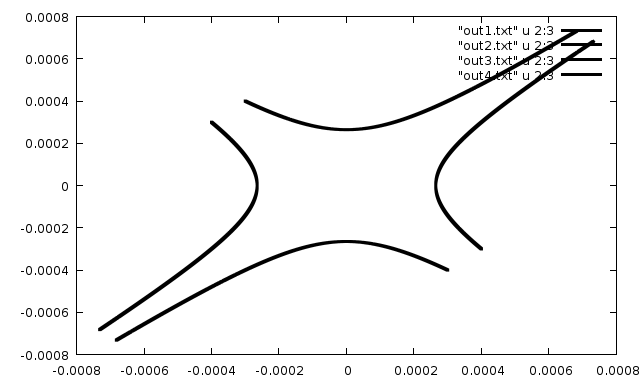
\includegraphics[width=1\textwidth]{all.png}
  \caption{Для особой точки $(0,0)$\label{first}}
\end{figure}

Моделирование вблизи точек $(1,0)$ и $(0,0)$. Результат на рис. \ref{second}. Моделиворание подтвердило характер фазовых кривых вблизи особой точки. Фазовая траектория --- <<седло>> гиперболы.
\begin{figure}[!h]
  \centering
  \includegraphics[width=1\textwidth]{2.png}
  \caption{Для особых точек $(1,0)$ и $(0,0)$\label{second}}
\end{figure}

%Моделирование общей фазовой картины. Результат на рис. \ref{third}.
\newpage
\section{Вывод}
В ходе данной лабораторной работы я научился обезразмеривать функции, определять особые точки динамической системы, заданной дифференциальной моделью 2-го порядка, и их характер.
\end{document}
